\documentclass[twoside]{article}

% Packages required by doxygen
\usepackage{fixltx2e}
\usepackage{calc}
\usepackage{doxygen}
\usepackage[export]{adjustbox} % also loads graphicx
\usepackage{graphicx}
\usepackage[utf8]{inputenc}
\usepackage{makeidx}
\usepackage{multicol}
\usepackage{multirow}
\PassOptionsToPackage{warn}{textcomp}
\usepackage{textcomp}
\usepackage[nointegrals]{wasysym}
\usepackage[table]{xcolor}

% NLS support packages
\usepackage{polski}
\usepackage[T1]{fontenc}

% Font selection
\usepackage[T1]{fontenc}
\usepackage[scaled=.90]{helvet}
\usepackage{courier}
\usepackage{amssymb}
\usepackage{sectsty}
\renewcommand{\familydefault}{\sfdefault}
\allsectionsfont{%
  \fontseries{bc}\selectfont%
  \color{darkgray}%
}
\renewcommand{\DoxyLabelFont}{%
  \fontseries{bc}\selectfont%
  \color{darkgray}%
}
\newcommand{\+}{\discretionary{\mbox{\scriptsize$\hookleftarrow$}}{}{}}

% Page & text layout
\usepackage{geometry}
\geometry{%
  a4paper,%
  top=2.5cm,%
  bottom=2.5cm,%
  left=2.5cm,%
  right=2.5cm%
}
\tolerance=750
\hfuzz=15pt
\hbadness=750
\setlength{\emergencystretch}{15pt}
\setlength{\parindent}{0cm}
\setlength{\parskip}{0.2cm}
\makeatletter
\renewcommand{\paragraph}{%
  \@startsection{paragraph}{4}{0ex}{-1.0ex}{1.0ex}{%
    \normalfont\normalsize\bfseries\SS@parafont%
  }%
}
\renewcommand{\subparagraph}{%
  \@startsection{subparagraph}{5}{0ex}{-1.0ex}{1.0ex}{%
    \normalfont\normalsize\bfseries\SS@subparafont%
  }%
}
\makeatother

% Headers & footers
\usepackage{fancyhdr}
\pagestyle{fancyplain}
\fancyhead[LE]{\fancyplain{}{\bfseries\thepage}}
\fancyhead[CE]{\fancyplain{}{}}
\fancyhead[RE]{\fancyplain{}{\bfseries\leftmark}}
\fancyhead[LO]{\fancyplain{}{\bfseries\rightmark}}
\fancyhead[CO]{\fancyplain{}{}}
\fancyhead[RO]{\fancyplain{}{\bfseries\thepage}}
\fancyfoot[LE]{\fancyplain{}{}}
\fancyfoot[CE]{\fancyplain{}{}}
\fancyfoot[RE]{\fancyplain{}{\bfseries\scriptsize Wygenerowano Śr, 11 mar 2015 15\+:40\+:34 dla Laboratorium 1 programem Doxygen }}
\fancyfoot[LO]{\fancyplain{}{\bfseries\scriptsize Wygenerowano Śr, 11 mar 2015 15\+:40\+:34 dla Laboratorium 1 programem Doxygen }}
\fancyfoot[CO]{\fancyplain{}{}}
\fancyfoot[RO]{\fancyplain{}{}}
\renewcommand{\footrulewidth}{0.4pt}
\renewcommand{\sectionmark}[1]{%
  \markright{\thesection\ #1}%
}

% Indices & bibliography
\usepackage{natbib}
\usepackage[titles]{tocloft}
\setcounter{tocdepth}{3}
\setcounter{secnumdepth}{5}
\makeindex

% Hyperlinks (required, but should be loaded last)
\usepackage{ifpdf}
\ifpdf
  \usepackage[pdftex,pagebackref=true]{hyperref}
\else
  \usepackage[ps2pdf,pagebackref=true]{hyperref}
\fi
\hypersetup{%
  colorlinks=true,%
  linkcolor=blue,%
  citecolor=blue,%
  unicode%
}

% Custom commands
\newcommand{\clearemptydoublepage}{%
  \newpage{\pagestyle{empty}\cleardoublepage}%
}


%===== C O N T E N T S =====

\begin{document}

% Titlepage & ToC
\hypersetup{pageanchor=false,
             bookmarks=true,
             bookmarksnumbered=true,
             pdfencoding=unicode
            }
\pagenumbering{roman}
\begin{titlepage}
\vspace*{7cm}
\begin{center}%
{\Large Laboratorium 1 \\[1ex]\large 1.\+0 }\\
\vspace*{1cm}
{\large Wygenerowano przez Doxygen 1.8.9.1}\\
\vspace*{0.5cm}
{\small Śr, 11 mar 2015 15:40:34}\\
\end{center}
\end{titlepage}
\tableofcontents
\pagenumbering{arabic}
\hypersetup{pageanchor=true}

%--- Begin generated contents ---
\section{Program sluzacy do pomiaru zlozonosci obliczeniowej.}
\label{index}\hypertarget{index}{}\begin{DoxyAuthor}{Autor}
Wojcich Makuch 
\end{DoxyAuthor}
\begin{DoxyDate}{Data}
10.\+03.\+2015 
\end{DoxyDate}
\begin{DoxyVersion}{Wersja}
1.\+0
\end{DoxyVersion}
Zadaniem programu jest wygenerowanie tablic liczb pseldoloswych oraz pomiar zlozonosci obliczeniowej polegajacej na wymnozeniu kazdego z tych elementow przez 2. Program zapisuje dane w pliku o nazwie Pomiar\+Czasu1.\+txt.\hypertarget{index_wartosci}{}\subsection{wartosci}\label{index_wartosci}
Program wykonuje obliczenia dla tablic o rozmiarach\+: 10 50 1e02 5e02 1e03 5e03 1e04 5e04 1e06 2.\+5e06 5e06 7.\+5e06 1e07 5e07 1e08 2.\+5e08 
\section{Indeks klas}
\subsection{Lista klas}
Tutaj znajdują się klasy, struktury, unie i interfejsy wraz z ich krótkimi opisami\+:\begin{DoxyCompactList}
\item\contentsline{section}{\hyperlink{class_kolejka}{Kolejka$<$ typ $>$} \\*Definicja klasy \hyperlink{class_kolejka}{Kolejka} Zbudowana na tablicy posiada indeksy pokazujace na poczatek i na koniec kolejki. Zbudowana na szablonie }{\pageref{class_kolejka}}{}
\item\contentsline{section}{\hyperlink{class_lista}{Lista$<$ typ $>$} \\*Definicja klasy \hyperlink{class_lista}{Lista} Przechowuje obiekt oraz wskaznik na nastepny i pole rozmiar. Zbudowana na szablonie }{\pageref{class_lista}}{}
\item\contentsline{section}{\hyperlink{class_stos}{Stos$<$ typ $>$} \\*Definicja klasy \hyperlink{class_stos}{Stos} zedfiniowany za pomoca tablicy. Klasa zbudowana na szablonie }{\pageref{class_stos}}{}
\end{DoxyCompactList}

\section{Indeks plików}
\subsection{Lista plików}
Tutaj znajduje się lista wszystkich plików z ich krótkimi opisami\+:\begin{DoxyCompactList}
\item\contentsline{section}{\hyperlink{generuj_8cpp}{generuj.\+cpp} }{\pageref{generuj_8cpp}}{}
\item\contentsline{section}{\hyperlink{generuj_8hh}{generuj.\+hh} }{\pageref{generuj_8hh}}{}
\item\contentsline{section}{\hyperlink{main_8cpp}{main.\+cpp} }{\pageref{main_8cpp}}{}
\end{DoxyCompactList}

\section{Dokumentacja klas}
\hypertarget{classdane}{}\subsection{Dokumentacja klasy dane}
\label{classdane}\index{dane@{dane}}


{\ttfamily \#include $<$generuj.\+hh$>$}

\subsubsection*{Metody publiczne}
\begin{DoxyCompactItemize}
\item 
\hyperlink{classdane_a343d935dd2271b07694c830de41a3479}{dane} (long int wielkosc)
\item 
\hyperlink{classdane_ae013323d9e999cb4bd3a7fdbf51c4401}{$\sim$dane} ()
\item 
void \hyperlink{classdane_a3c63af736de15303e468404b892ff749}{generuj} ()
\item 
int \hyperlink{classdane_a9ae56a861bc8e17b33eaa92feba8fab7}{Wez} (int i) const 
\item 
int \hyperlink{classdane_a86a56a87d2cb77716fae2e0ff753ef82}{Wez\+Rozmiar} () const 
\item 
int \hyperlink{classdane_a97c3ef4d2c3cde0e701e30122c8c22fc}{Zapisz\+Do\+Pliku} (const char $\ast$nazwa)
\item 
double \hyperlink{classdane_ad217ab46050e5f3a16d92e69056e75f4}{licz} ()
\end{DoxyCompactItemize}
\subsubsection*{Atrybuty prywatne}
\begin{DoxyCompactItemize}
\item 
long int $\ast$ \hyperlink{classdane_a99cb90f61c23e390b594c688bd52ebf5}{tablica}
\item 
long int \hyperlink{classdane_abc9b63b1b2caa22fd4c71a8504d01ae6}{rozmiar}
\end{DoxyCompactItemize}


\subsubsection{Opis szczegółowy}
Klasa modeluje pojecie zbioru danych. Jej artybutem jest generowanie liczb pseldolosowych z zakresu 0-\/9 oraz pomiar zlozonosci obliczeniowej bazujacej na tych liczbach. 

Definicja w linii 23 pliku generuj.\+hh.



\subsubsection{Dokumentacja konstruktora i destruktora}
\hypertarget{classdane_a343d935dd2271b07694c830de41a3479}{}\index{dane@{dane}!dane@{dane}}
\index{dane@{dane}!dane@{dane}}
\paragraph[{dane}]{\setlength{\rightskip}{0pt plus 5cm}dane\+::dane (
\begin{DoxyParamCaption}
\item[{long int}]{wielkosc}
\end{DoxyParamCaption}
)\hspace{0.3cm}{\ttfamily [inline]}}\label{classdane_a343d935dd2271b07694c830de41a3479}

\begin{DoxyParams}[1]{Parametry}
\mbox{\tt in}  & {\em wielkosc} & -\/ liczba elementow tablicy, dla ktorej zostanie przydzielona pamiec. \\
\hline
\end{DoxyParams}


Definicja w linii 33 pliku generuj.\+hh.

\hypertarget{classdane_ae013323d9e999cb4bd3a7fdbf51c4401}{}\index{dane@{dane}!````~dane@{$\sim$dane}}
\index{````~dane@{$\sim$dane}!dane@{dane}}
\paragraph[{$\sim$dane}]{\setlength{\rightskip}{0pt plus 5cm}dane\+::$\sim$dane (
\begin{DoxyParamCaption}
{}
\end{DoxyParamCaption}
)\hspace{0.3cm}{\ttfamily [inline]}}\label{classdane_ae013323d9e999cb4bd3a7fdbf51c4401}


Definicja w linii 34 pliku generuj.\+hh.



\subsubsection{Dokumentacja funkcji składowych}
\hypertarget{classdane_a3c63af736de15303e468404b892ff749}{}\index{dane@{dane}!generuj@{generuj}}
\index{generuj@{generuj}!dane@{dane}}
\paragraph[{generuj}]{\setlength{\rightskip}{0pt plus 5cm}void dane\+::generuj (
\begin{DoxyParamCaption}
{}
\end{DoxyParamCaption}
)}\label{classdane_a3c63af736de15303e468404b892ff749}
wypelnia tablice liczbami pseldolosowymi z zakresu 0-\/9. 

Definicja w linii 27 pliku generuj.\+cpp.

\hypertarget{classdane_ad217ab46050e5f3a16d92e69056e75f4}{}\index{dane@{dane}!licz@{licz}}
\index{licz@{licz}!dane@{dane}}
\paragraph[{licz}]{\setlength{\rightskip}{0pt plus 5cm}double dane\+::licz (
\begin{DoxyParamCaption}
{}
\end{DoxyParamCaption}
)}\label{classdane_ad217ab46050e5f3a16d92e69056e75f4}
Wykonuje operacje na tablicy polegajace na wymnozeniu kazdego elementu przez 2. Mierzy czas wykonywanych operacji z dokladnoscia do e-\/06s. \begin{DoxyReturn}{Zwraca}
tm -\/ zmierzony czas. 
\end{DoxyReturn}


Definicja w linii 35 pliku generuj.\+cpp.

\hypertarget{classdane_a9ae56a861bc8e17b33eaa92feba8fab7}{}\index{dane@{dane}!Wez@{Wez}}
\index{Wez@{Wez}!dane@{dane}}
\paragraph[{Wez}]{\setlength{\rightskip}{0pt plus 5cm}int dane\+::\+Wez (
\begin{DoxyParamCaption}
\item[{int}]{i}
\end{DoxyParamCaption}
) const\hspace{0.3cm}{\ttfamily [inline]}}\label{classdane_a9ae56a861bc8e17b33eaa92feba8fab7}

\begin{DoxyParams}[1]{Parametry}
\mbox{\tt in}  & {\em i} & -\/ indeks tablicy. \\
\hline
\end{DoxyParams}
\begin{DoxyReturn}{Zwraca}
zwraca element tablicy. 
\end{DoxyReturn}


Definicja w linii 46 pliku generuj.\+hh.

\hypertarget{classdane_a86a56a87d2cb77716fae2e0ff753ef82}{}\index{dane@{dane}!Wez\+Rozmiar@{Wez\+Rozmiar}}
\index{Wez\+Rozmiar@{Wez\+Rozmiar}!dane@{dane}}
\paragraph[{Wez\+Rozmiar}]{\setlength{\rightskip}{0pt plus 5cm}int dane\+::\+Wez\+Rozmiar (
\begin{DoxyParamCaption}
{}
\end{DoxyParamCaption}
) const\hspace{0.3cm}{\ttfamily [inline]}}\label{classdane_a86a56a87d2cb77716fae2e0ff753ef82}
\begin{DoxyReturn}{Zwraca}
Zwraca rozmiar tablicy. 
\end{DoxyReturn}


Definicja w linii 51 pliku generuj.\+hh.

\hypertarget{classdane_a97c3ef4d2c3cde0e701e30122c8c22fc}{}\index{dane@{dane}!Zapisz\+Do\+Pliku@{Zapisz\+Do\+Pliku}}
\index{Zapisz\+Do\+Pliku@{Zapisz\+Do\+Pliku}!dane@{dane}}
\paragraph[{Zapisz\+Do\+Pliku}]{\setlength{\rightskip}{0pt plus 5cm}int dane\+::\+Zapisz\+Do\+Pliku (
\begin{DoxyParamCaption}
\item[{const char $\ast$}]{nazwa}
\end{DoxyParamCaption}
)}\label{classdane_a97c3ef4d2c3cde0e701e30122c8c22fc}
Zapisuje elementy tablicy w pliku o zadanej nazwie. 
\begin{DoxyParams}[1]{Parametry}
\mbox{\tt in}  & {\em nazwa} & -\/ nazwa pliku do zapisu. \\
\hline
\end{DoxyParams}
\begin{DoxyReturn}{Zwraca}
0 -\/ Poprawny zapis. -\/1 -\/ Niepoprawny zapis. 
\end{DoxyReturn}


Definicja w linii 60 pliku generuj.\+cpp.



\subsubsection{Dokumentacja atrybutów składowych}
\hypertarget{classdane_abc9b63b1b2caa22fd4c71a8504d01ae6}{}\index{dane@{dane}!rozmiar@{rozmiar}}
\index{rozmiar@{rozmiar}!dane@{dane}}
\paragraph[{rozmiar}]{\setlength{\rightskip}{0pt plus 5cm}long int dane\+::rozmiar\hspace{0.3cm}{\ttfamily [private]}}\label{classdane_abc9b63b1b2caa22fd4c71a8504d01ae6}


Definicja w linii 26 pliku generuj.\+hh.

\hypertarget{classdane_a99cb90f61c23e390b594c688bd52ebf5}{}\index{dane@{dane}!tablica@{tablica}}
\index{tablica@{tablica}!dane@{dane}}
\paragraph[{tablica}]{\setlength{\rightskip}{0pt plus 5cm}long int$\ast$ dane\+::tablica\hspace{0.3cm}{\ttfamily [private]}}\label{classdane_a99cb90f61c23e390b594c688bd52ebf5}


Definicja w linii 25 pliku generuj.\+hh.



Dokumentacja dla tej klasy została wygenerowana z plików\+:\begin{DoxyCompactItemize}
\item 
\hyperlink{generuj_8hh}{generuj.\+hh}\item 
\hyperlink{generuj_8cpp}{generuj.\+cpp}\end{DoxyCompactItemize}

\section{Dokumentacja plików}
\hypertarget{generuj_8cpp}{}\subsection{Dokumentacja pliku generuj.\+cpp}
\label{generuj_8cpp}\index{generuj.\+cpp@{generuj.\+cpp}}
{\ttfamily \#include $<$iostream$>$}\\*
{\ttfamily \#include $<$fstream$>$}\\*
{\ttfamily \#include $<$cstdlib$>$}\\*
{\ttfamily \#include $<$conio.\+h$>$}\\*
{\ttfamily \#include $<$ctime$>$}\\*
{\ttfamily \#include \char`\"{}generuj.\+hh\char`\"{}}\\*
\subsubsection*{Funkcje}
\begin{DoxyCompactItemize}
\item 
L\+A\+R\+G\+E\+\_\+\+I\+N\+T\+E\+G\+E\+R \hyperlink{generuj_8cpp_a4fbb2a5fceb3efd577419fc87c6f3d07}{start\+Timer} ()
\item 
L\+A\+R\+G\+E\+\_\+\+I\+N\+T\+E\+G\+E\+R \hyperlink{generuj_8cpp_abd320a48742faf3aa6ad1a7e7c6b518b}{end\+Timer} ()
\end{DoxyCompactItemize}


\subsubsection{Dokumentacja funkcji}
\hypertarget{generuj_8cpp_abd320a48742faf3aa6ad1a7e7c6b518b}{}\index{generuj.\+cpp@{generuj.\+cpp}!end\+Timer@{end\+Timer}}
\index{end\+Timer@{end\+Timer}!generuj.\+cpp@{generuj.\+cpp}}
\paragraph[{end\+Timer}]{\setlength{\rightskip}{0pt plus 5cm}L\+A\+R\+G\+E\+\_\+\+I\+N\+T\+E\+G\+E\+R end\+Timer (
\begin{DoxyParamCaption}
{}
\end{DoxyParamCaption}
)}\label{generuj_8cpp_abd320a48742faf3aa6ad1a7e7c6b518b}
Funkcja konczy pomiar czasu \begin{DoxyReturn}{Zwraca}
koniec -\/ zmierzony czas 
\end{DoxyReturn}


Definicja w linii 17 pliku generuj.\+cpp.

\hypertarget{generuj_8cpp_a4fbb2a5fceb3efd577419fc87c6f3d07}{}\index{generuj.\+cpp@{generuj.\+cpp}!start\+Timer@{start\+Timer}}
\index{start\+Timer@{start\+Timer}!generuj.\+cpp@{generuj.\+cpp}}
\paragraph[{start\+Timer}]{\setlength{\rightskip}{0pt plus 5cm}L\+A\+R\+G\+E\+\_\+\+I\+N\+T\+E\+G\+E\+R start\+Timer (
\begin{DoxyParamCaption}
{}
\end{DoxyParamCaption}
)}\label{generuj_8cpp_a4fbb2a5fceb3efd577419fc87c6f3d07}
Funcja rozpoczyna pomiar czasu. \begin{DoxyReturn}{Zwraca}
start -\/ zmierzony czas. 
\end{DoxyReturn}


Definicja w linii 9 pliku generuj.\+cpp.


\hypertarget{generuj_8hh}{}\subsection{Dokumentacja pliku generuj.\+hh}
\label{generuj_8hh}\index{generuj.\+hh@{generuj.\+hh}}
{\ttfamily \#include $<$Windows.\+h$>$}\\*
\subsubsection*{Komponenty}
\begin{DoxyCompactItemize}
\item 
class \hyperlink{classdane}{dane}
\end{DoxyCompactItemize}
\subsubsection*{Funkcje}
\begin{DoxyCompactItemize}
\item 
L\+A\+R\+G\+E\+\_\+\+I\+N\+T\+E\+G\+E\+R \hyperlink{generuj_8hh_a4fbb2a5fceb3efd577419fc87c6f3d07}{start\+Timer} ()
\item 
L\+A\+R\+G\+E\+\_\+\+I\+N\+T\+E\+G\+E\+R \hyperlink{generuj_8hh_abd320a48742faf3aa6ad1a7e7c6b518b}{end\+Timer} ()
\end{DoxyCompactItemize}


\subsubsection{Dokumentacja funkcji}
\hypertarget{generuj_8hh_abd320a48742faf3aa6ad1a7e7c6b518b}{}\index{generuj.\+hh@{generuj.\+hh}!end\+Timer@{end\+Timer}}
\index{end\+Timer@{end\+Timer}!generuj.\+hh@{generuj.\+hh}}
\paragraph[{end\+Timer}]{\setlength{\rightskip}{0pt plus 5cm}L\+A\+R\+G\+E\+\_\+\+I\+N\+T\+E\+G\+E\+R end\+Timer (
\begin{DoxyParamCaption}
{}
\end{DoxyParamCaption}
)}\label{generuj_8hh_abd320a48742faf3aa6ad1a7e7c6b518b}
Funkcja konczy pomiar czasu \begin{DoxyReturn}{Zwraca}
koniec -\/ zmierzony czas 
\end{DoxyReturn}


Definicja w linii 14 pliku generuj.\+cpp.

\hypertarget{generuj_8hh_a4fbb2a5fceb3efd577419fc87c6f3d07}{}\index{generuj.\+hh@{generuj.\+hh}!start\+Timer@{start\+Timer}}
\index{start\+Timer@{start\+Timer}!generuj.\+hh@{generuj.\+hh}}
\paragraph[{start\+Timer}]{\setlength{\rightskip}{0pt plus 5cm}L\+A\+R\+G\+E\+\_\+\+I\+N\+T\+E\+G\+E\+R start\+Timer (
\begin{DoxyParamCaption}
{}
\end{DoxyParamCaption}
)}\label{generuj_8hh_a4fbb2a5fceb3efd577419fc87c6f3d07}
Funcja rozpoczyna pomiar czasu. \begin{DoxyReturn}{Zwraca}
start -\/ zmierzony czas. 
\end{DoxyReturn}


Definicja w linii 6 pliku generuj.\+cpp.


\hypertarget{main_8cpp}{}\subsection{Dokumentacja pliku main.\+cpp}
\label{main_8cpp}\index{main.\+cpp@{main.\+cpp}}
{\ttfamily \#include $<$iostream$>$}\\*
{\ttfamily \#include $<$windows.\+h$>$}\\*
{\ttfamily \#include $<$fstream$>$}\\*
{\ttfamily \#include \char`\"{}generuj.\+hh\char`\"{}}\\*
\subsubsection*{Funkcje}
\begin{DoxyCompactItemize}
\item 
int \hyperlink{main_8cpp_ae66f6b31b5ad750f1fe042a706a4e3d4}{main} ()
\end{DoxyCompactItemize}


\subsubsection{Dokumentacja funkcji}
\hypertarget{main_8cpp_ae66f6b31b5ad750f1fe042a706a4e3d4}{}\index{main.\+cpp@{main.\+cpp}!main@{main}}
\index{main@{main}!main.\+cpp@{main.\+cpp}}
\paragraph[{main}]{\setlength{\rightskip}{0pt plus 5cm}int main (
\begin{DoxyParamCaption}
{}
\end{DoxyParamCaption}
)}\label{main_8cpp_ae66f6b31b5ad750f1fe042a706a4e3d4}


Definicja w linii 26 pliku main.\+cpp.


\documentclass[8pt,a4paper]{article}
\usepackage{polski}
\usepackage[utf8]{inputenc}
\usepackage{graphicx}

\author{Wojciech Makuch}
\date{11.03.2015}
\title{Laboratorium 1}

\begin{document}
	\maketitle
	\begin{enumerate}
		\item{Zadanie} \\
		Napisać program generujący liczby psełdolosowe, a nastepnie liczący złożonosć obliczeniową wymnożenia każdego z tych elementów przez~2.
		\item{Realizacja} \\
		Program zawiera jedną klase przechowującą rozmiar oraz liczby psełdolowe. Klasa zawiera metody wypęłniające tablice, mnożące każdy z elementów przez 2, zliczając przy tym czas wykonania tej operacji. Ponadto program ma możliwość zapisania danych do pliku. Program nie posiada interfejsu z użytkownikiem.
		\item{Działanie} \\
		Główna funckja programu zawiera 18 objektów. Każdy z nich posiada inny rozmiar. Program po kolei inicjuje objekty, liczy złożoność obliczeniową, następnie wyświetla wynik na ekranie oraz zapisuje do pliku.
		\item{Wykres zależnosci ilosci obliczeń od czasu} \\ 
		\\
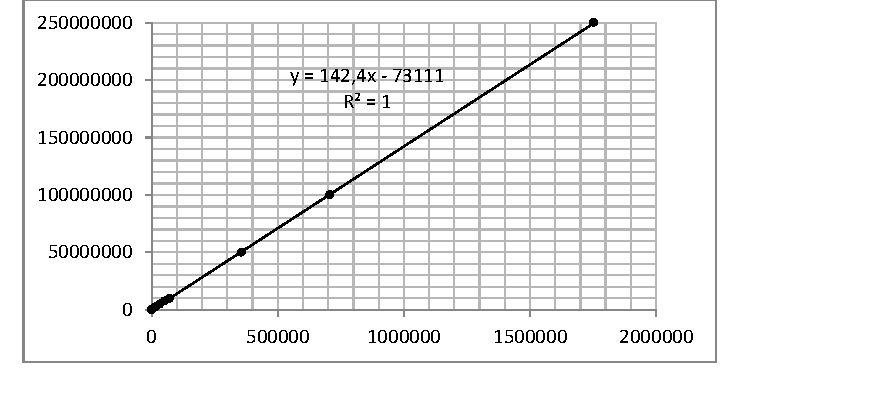
\includegraphics{Dok1.pdf}	
		\item{Komentarz} \\
		Do utworzenia dokumentacji wykorzystano system Doxygen.
		Funkcja pomiaru czasu dla systemu Windows pobrana ze strony dr. J. Mierzwy. Program skompilowano w środowisku Code::Blocks. Do stworzonia wykresu posłużono się pakietem MS Excel, sprawozdanie napisano uzywając systemu \LaTeX.
	\end{enumerate}
\end{document}